\documentclass[oneside,12pt,a4paper]{template/SPSTemplate} % Default font size is 12pt, it can be changed here

\usepackage{graphicx}
\usepackage{amsmath} % mathematical fractions
\usepackage{lipsum}
\usepackage{float}
\usepackage{biblatex}  %  sudo apt-get install texlive-bibtex-extra
\addbibresource{zdroje.bib}
\graphicspath{{./template/}{./Pictures/}}

\creator{VERNER Adam}
\temacz{Dvoukanálový USB osciloskop}
\tema{Two-channel USB oscilloscope}
\supervisor{BUŠEK Jaroslav}
\vyuziti{Výukové účely v oboru mechatronika, programování, digitální zpracování signálu}
\abstrakt{Práce je zaměřena na vývoj zařízení sloužícího k digitálnímu zpracování analogového signálu}
\klicovas{Osciloskop, SystemVerilog, FPGA, USB, ADC, Pyhon, GTK, Altera}
\usage{Teaching purposes in the field of mechatronics, programming and digital signal processing}
\abstrakten{This work is focused on development of device used to digitally process an analogue signal}
\keywords{Oscilloscope, SystenVerilog, FPGA, USB, ADC, Python, GTK, Altera}
\podekovani{Děkuji vedoucímu práce za nulovou důvěru v mojí schopnost řádného dokončení projektu, která mě motivovala udělat něco víc, než všichni očekávají.\\
Také bych chtěl poděkovat svému otci, který mě již v útlém věku zainteresoval do digitálního světa, tím, že mě nechal rozbíjet vyřazené počítače.}


\begin{document}
	\makebeginning

	\addcontentsline{toc}{chapter}{Obsah}
	\tableofcontents

	
	\chapter{Úvod}
	
	\chapter{Analogově digitální převodníky}
	\section{Vzorkování}
	Ve zpracování signálu se vzorkováním myslí převod časově spojitého signálu do oblasti diskrétního
	času. "Odebírání vzorků" může být provedeno Vzorkování může být vyjádřeno buďto jako frekvence $ f_{vz} $ nebo jako perioda $ T_{vz} $.
	Závislost frekvence na periodě vzorkování je vyjádřena v následující rovnici:
	
	\begin{equation}
	f_{vz} = \frac{1}{T_{vz}}
	\end{equation}

	
	\subsection{Aliasing}
	Vycházející z anglického slova \textit{alias}, znamenající: falešné jméno, pseudonym, "jinak zvaný." 
	

\textit{„Přesná rekonstrukce spojitého, frekvenčně omezeného signálu z jeho vzorků je možná tehdy, pokud byla vzorkovací frekvence vyšší než dvojnásobek nejvyšší harmonické složky vzorkovaného signálu.“}\cite{sampling_nyquist}
	
	\begin{figure}
		\centering
		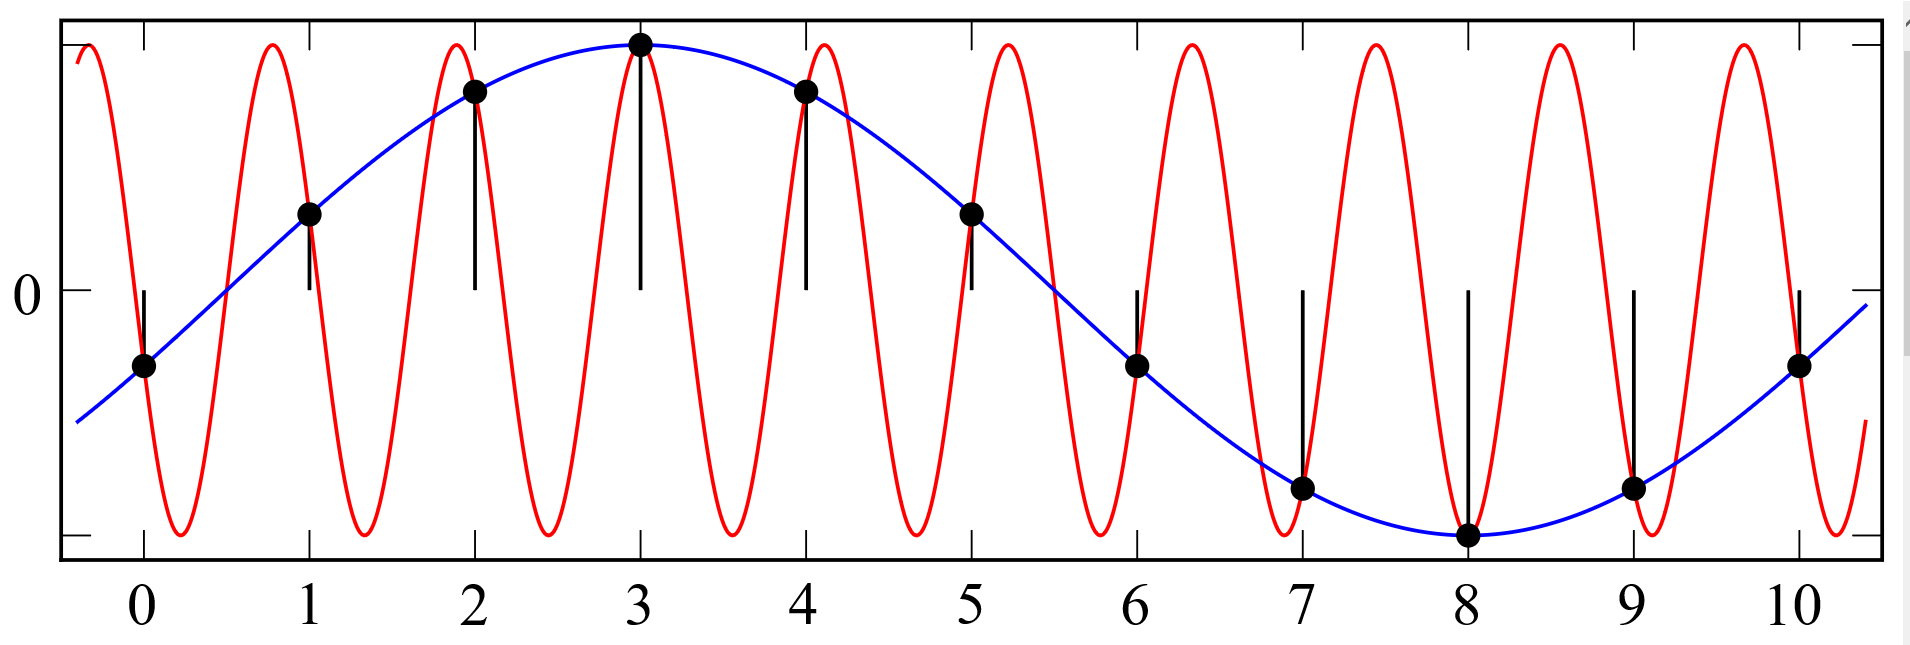
\includegraphics[width=\textwidth,keepaspectratio]{AliasingSines.eps}
		\caption{Červená - vzorkovaný signál. Modrá - rekonstruovaný signál}
		\label{img:aliasing}
	\end{figure}
	
	
	\appendix
	
	\printbibliography
	
	\listoffigures
	\listoftables
	

\end{document}

